\section{Durchführung}
\begin{figure}
    \centering
    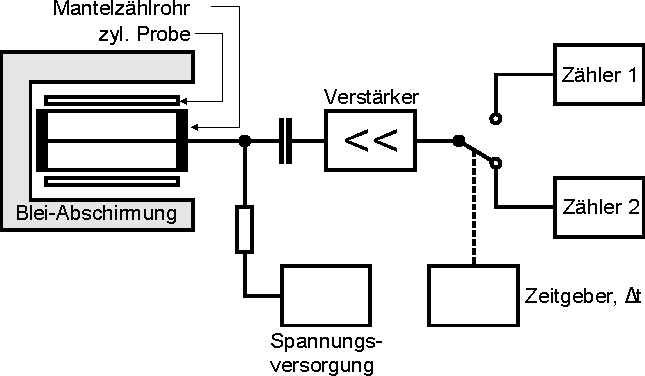
\includegraphics{Abbildungen/Schaltplan.pdf}
    \caption{Aufbau der Messanlage \cite{man:v702}}
    \label{fig:Aufbau}
\end{figure}
Die Messungen erfolgen mit der In Abb. \ref{fig:Aufbau} skizzierten Apparatur.
Mit einem Geiger-Müller-Zählrohr werden die von den Proben emittierten
$\beta$- und $\gamma$-Teilchen gemessen. 
Der Verstärker macht es möglich die gemessenen Teilchen 
in den Zählmaschinen zu zählen. 
In einer Angemessenen Zeit $\Delta t$ wird das Signal zwischen den
Zählmaschinen hin und her geschaltet.
Das Messgerät wird durch eine Bleiwand von der äusseren 
Hintergrundstrahlung abgeschirmt. 
Trotzdem existiert ein sogenannter Nulleffekt, Strahlung 
die ohne hinzufügen von einer Radioaktiven Strahlungsquelle gemessen werden kann.
Dieser Nulleffekt wird in der ersten Messreihe gemessen.
Bei dieser Messreihe wird ein $\delta t$ von \qty{35}{\s} gewählt. 
Anschliessend wird die Strahlung der in der Neutronenquelle (vgl. Abb. \ref{fig:neutronenquelle})
erzeugten radioaktiven Isotope gemessen.
Dazu werden die Zylinderförmigen Bleche aus der Neutronenquelle genommen und so schnell
wie möglich über das Geiger-Müller-Zählrohr geschoben.
Direkt danach wird die Messung gestartet.
Die geeigneten Zeitintervalle $\Delta t$ sind nur durch aufwändige vorherige Experimente zu ermitteln.
Zur besseren Durchführbarkeit der Experimente sind ideale Werte für $\Delta t$
und die Minimale Anregungszeit in der Neutronenquelle bereits vorgegeben.
In Tabelle \ref{tab:zeiten} werden die nach diesen Vorgaben verwendeten Zeiten
aufgelistet.
\begin{table}%
    \begin{tabular}{c c c c}%
        \toprule%
        Element  & $\delta T$ & Minimale Zeit in       & Dauer der\\%
                 &            & der Neutronenquelle    & Messreihe\\%
        \midrule        %
        Vanadium & \qty{35}{\s}   &  \qty{15}{\minute} & \qty{17}{\minute}\\%
        Silber   & \qty{10}{\s}   &  \qty{10}{\minute} & \qty{8}{\minute}\\%
    \end{tabular}%
    \caption{Verwendete Einstellungen für die Messreihen.}%
    \label{tab:zeiten}%
\end{table}%
Für die Silberprobe wird die gleiche Messung zweimal wiederholt um mit 
mehr Daten einen kleineren Messfehler zu erreichen.
